%% ============================================================
%%  Chapter 4 — Compositional and Chemical Control of Volatile
%%              Polymer-Electrolyte Memristive Dynamics
%%
%%  NOTE: bound as Chapter 4 (a bridge chapter precedes it as Ch3).
%%  Internal labels use the ch4_ prefix and figures live in
%%  figures/chapter4/, matching the bound order.
%%
%%  Author : Carlos David Prado-Socorro
%%  Date   : June 2026
%%  Institution : ICMol, Universitat de València
%%
%%  Compile with: latexmk -pdf  (standalone) or via thesis.tex
%%  Plan + evidence: handouts/10_chapter3_comparative_plan.md,
%%                   handouts/08_chapter3_4_claims_audit.md
%% ============================================================

%% ---- Standalone preamble (skipped when \include'd from thesis.tex) ----
\ifdefined\thesismode\else
  \documentclass[12pt, twoside]{report}
  \usepackage{thesis-format}
  \addbibresource{../bibliography/references.bib}
  \begin{document}
  \setcounter{chapter}{3}     % This is Chapter 4 when built standalone
\fi

%% --- Shared macros (\providecommand: harmless if ch.2 already declared them) ---
\providecommand{\SY}{\textit{Super Yellow}}
\providecommand{\Hybrane}{\textit{Hybrane}}
\providecommand{\PEO}{PEO}
\providecommand{\TMPE}{TMPE}
\providecommand{\LiTf}{LiOTf}
\providecommand{\NaTf}{NaOTf}
\providecommand{\KTf}{KOTf}
\providecommand{\TFSI}{TFSI}
\providecommand{\ITO}{ITO}
\providecommand{\twoterminal}{two-terminal}
%% Standalone-safe reference into this chapter's Supporting Information
%% (Appendix C). Resolves with \cref in the full thesis; prints a literal
%% label in standalone builds, where the appendix is not included.
\providecommand{\siCompRef}[1]{\ifdefined\thesismode\cref{#1}\else Appendix~C\fi}

%% ============================================================
\chapter{Compositional and Chemical Control of Volatile Polymer-Electrolyte Memristive Dynamics}\label{ch:comparative}
%% ============================================================

%% ------------------------------------------------------------
\section{Introduction and Scope}\label{sec:ch4_intro}
%% ------------------------------------------------------------

\Cref{ch:poc} established the memristive response of the \SY{}/\Hybrane{}/\LiTf{} formulation and 2-T architecture across assay-specific junctions. The broader device corpus examined here varies the composition, electrolyte chemistry, electrode, and drive protocol of the same three-component architecture.

Three families of measurement recur on the same 2-T geometry throughout this chapter and the next: (i) current--voltage hysteresis, which reports the steady-state switching window; (ii) potentiation as a function of the number of applied write pulses, which reports how the conductance is built up; and (iii) depotentiation as a function of the delay before read-out, which reports how a written state fades. Introduced as a named set in \cref{ch:poc}, they are the shared, abundant basis of the comparative work. The richer proof-of-concept synaptic protocols of \cref{ch:poc} (excitatory post-synaptic current, separated short- and long-term memory, and spike-timing dependent plasticity) are \emph{not} repeated here; where invoked, they serve only as formulation-level prior evidence.

\paragraph{Scope of the comparisons.} The \SY{}/\PEO{}/\LiTf{} composition grid contains typically two to four nominally identical devices per cell and supports quantitative comparisons. After data-quality screening, the host, anion, and cation contrasts contain at most one or two devices per matched cell and are used only as an illustrative survey. The electrode comparison is likewise illustrative and is available only at the lead composition (\cref{sec:ch4_electrode}). Drive protocol is analysed separately because it changes the apparent fading-memory timescale and therefore limits comparisons between protocols.

%% ------------------------------------------------------------
\section{Materials, Devices, and Measurement Protocol}\label{sec:ch4_materials}
%% ------------------------------------------------------------

The devices retain the architecture of \cref{ch:poc}: a vertical \twoterminal{} sandwich of \ITO{} (bottom, transparent), a solution-processed composite active layer, and a thermally evaporated silver top electrode, with a junction area of \SI{8.25e-2}{\centi\meter\squared}. \SY{} is retained as the semiconducting component in every device of this chapter, so that the electronic-transport role is held fixed and the variation is confined to the ion-transport phase.

The experiment varies composition and chemistry. The \emph{composition} axis changes the mass ratios of the ion-transport polymer poly(ethylene oxide) (\PEO{}) and lithium triflate salt (\LiTf{}) relative to the semiconductor: \(r_{\PEO{}}=m_{\PEO{}}/m_{\SY{}}\) and \(r_{\mathrm{salt}}=m_{\mathrm{salt}}/m_{\SY{}}\). These are blend-component ratios, not fractions of the total dry mass. The \emph{chemistry} axis substitutes the ion-transport host, the salt anion (triflate or bis(trifluoromethanesulfonyl)imide, \TFSI{}), and the alkali cation (\ce{Li+}, \ce{Na+}, \ce{K+}, as the triflate or \TFSI{} salt). The comparative work replaces the hyperbranched polyester-amide \Hybrane{} host of the proof-of-concept device (\cref{ch:poc}) with two hosts: linear \PEO{} and the hyperbranched polyether trimethylolpropane ethoxylate (\TMPE{}). This gives a matched-chemistry contrast between linear and branched polyethers. Every device reported \emph{quantitatively} uses the silver electrode. A separate gold-electrode corpus at the lead composition compares an active with an inert electrode, measures drive-polarity dependence on gold, and provides an independent-electrode check on the chemistry comparisons (\cref{sec:ch4_electrode}).

\paragraph{Control for film thickness.} Adding ion-transport polymer thickens the solution-processed film, so most higher-\PEO{} cells were spun faster to reduce thickness differences across the grid (\SIrange{1500}{3500}{rpm}). This compensation was incomplete and was not applied uniformly to every comparison batch. In the silver composition series (\(n=30\)), median thickness rises from \(\approx\SI{227}{\nano\meter}\) at \PEO{}~\num{0.3} to \(\approx\SI{298}{\nano\meter}\) at \PEO{}~\num{1.2} (Pearson \(r\approx0.68\); \cref{fig:ch4_thickness_control}). Several controls separate this covariation from the composition result. The reported responses are dimensionless ratios or timescales; activation voltage remains within \SIrange{2.2}{2.4}{\volt} across the full \(2.6\times\) thickness range (\(r\approx-0.06\)); and a \(38\%\) within-cell thickness spread leaves the fading-memory time essentially unchanged. The partial correlation between thickness and \(\log t_{1/2}\), controlling for \PEO{}, is \(\approx+0.05\), whereas the association with composition, controlling for thickness, is \(\approx-0.42\). Thus, thickness covaries with polymer loading, while the dynamics retain an association with composition after thickness control. Full statistics and the audit of other fabrication variables are given in \siCompRef{app:ch4_confounds}.

\begin{figure}[t]
  \centering
  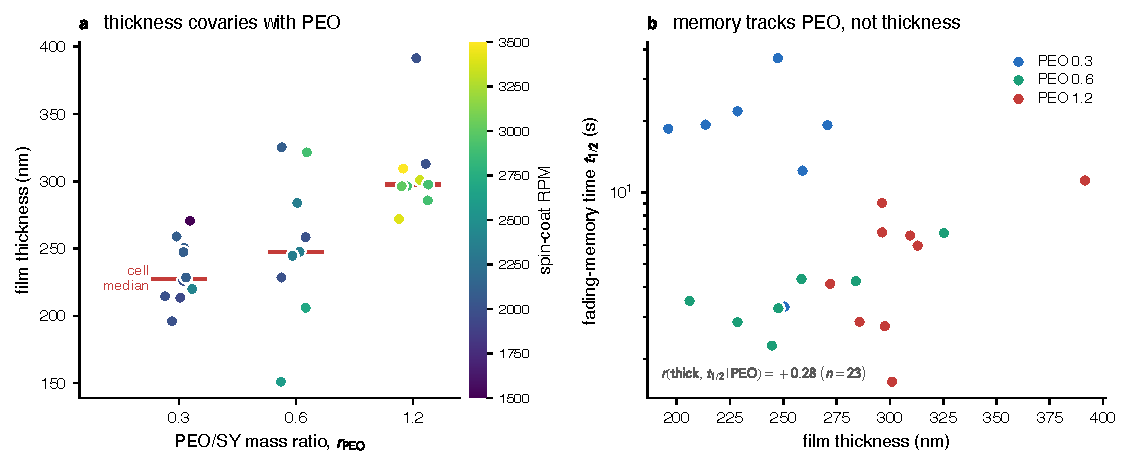
\includegraphics[width=\linewidth]{../figures/chapter4/thickness_control.pdf}
  \caption[Film-thickness control]{Film thickness and fading-memory time in the silver composition series (\(n=30\)). (a)~Film thickness rises with \(r_{\PEO{}}\) (red bars are cell medians); higher-\PEO{} cells were spun faster (colour) to reduce this difference, although residual covariation remains. (b)~Within each \(r_{\PEO{}}\) band, \(t_{1/2}\) is approximately flat against thickness; the partial correlation between thickness and \(t_{1/2}\), controlling for \(r_{\PEO{}}\), is \(\approx 0\).}
  \label{fig:ch4_thickness_control}
\end{figure}

\paragraph{Drive and read protocols.} Because the comparisons below turn on them, the electrical protocols are stated explicitly, and they are \emph{not} identical across the three measurements (\cref{tab:ch4_protocols}). Hysteresis uses a triangular voltage sweep. The potentiation ($N$-pulse build-up) was acquired with a \SI{3}{\volt} write and \SI{1.5}{\volt} read at a variable pulse count ($N\le\num{1000}$); the depotentiation (fading-memory decay) used a fixed train of \num{30} write pulses at a \SI{4}{\volt} write and \SI{2}{\volt} read. The inter-pulse interval is effectively common (\SI{0.104}{\second} for potentiation, \SI{0.103}{\second} for depotentiation), but the \emph{write amplitude differs} between the two (\SI{3}{\volt} vs \SI{4}{\volt}), a point that matters when the two are later composed (\cref{sec:ch4_limitations}, \Cref{ch:temporal}). The read voltage is above the ionic activation threshold established in \cref{ch:poc}, a point returned to in \cref{sec:ch4_protocol}. An older 2022 device generation used a \SI{6}{\volt} write with a \SI{3}{\volt} read; the modern and old amplitudes are never pooled, and the same-device contrast between two amplitudes is itself the drive-protocol result (\cref{sec:ch4_protocol}).

\begin{table}[t]
  \centering
  \caption[Electrical measurement protocols]{The three common measurements use distinct drive protocols (modern \SY{}/\PEO{}/\LiTf{}/Ag corpus). Potentiation and depotentiation differ in write amplitude, so the chapter never pools them and \Cref{ch:temporal} composes them only as an explicit assumption.}
  \label{tab:ch4_protocols}
  {\small\setlength{\tabcolsep}{3pt}%
  \begin{tabular}{@{}lll >{\raggedright\arraybackslash}p{2.45cm}@{}}
    \toprule
    Measurement & Write & Read & Pulse train \\
    \midrule
    Hysteresis (HYST)          & triangular sweep            & ---                            & ---                                   \\
    Potentiation (PULSES)      & \SI{3}{\volt}               & \SI{1.5}{\volt}                & variable $N\le\num{1000}$, \SI{0.104}{\second} \\
    Depotentiation (DELAYTIME) & \SI{4}{\volt}               & \SI{2}{\volt}                  & \num{30} pulses, \SI{0.103}{\second}  \\
    Protocol overlay (v114)    & \SI{3}{\volt}, \SI{6}{\volt} & \SI{1.5}{\volt}, \SI{3}{\volt} & \num{30} pulses                       \\
    \bottomrule
  \end{tabular}}
\end{table}

%% ------------------------------------------------------------
\section{Methods of Analysis}\label{sec:ch4_methods}
%% ------------------------------------------------------------

Hysteresis curves are summarised by the on--off conductance ratio and by a normalised loop area; potentiation curves by the per-decade growth of the conductance ratio with pulse number, by the peak ratio, and by whether the response turns over (decreases) at the highest pulse counts; and depotentiation curves by a fading-memory time constant.

For the depotentiation (fading-memory) decay, the comparative archive is refitted with the more general Kohlrausch (stretched-exponential) function
\begin{equation}
  \label{eq:ch4_kohlrausch}
  \Delta G(t_{\mathrm{wait}}) = \Delta G_0\,\exp\!\left[-\left(\frac{t_{\mathrm{wait}}}{\tau}\right)^{\beta}\right] + \Delta G_\infty,
\end{equation}
with characteristic relaxation time \(\tau\), stretch exponent \(0 < \beta \le 1\), initial change \(\Delta G_0\), and residual \(\Delta G_\infty\)~\cite{Sturman2003}. The eight-to-thirteen-point decay curves often under-constrain \(\beta\) and \(\tau\) jointly. The fitted \(\tau\) is therefore reported only where the fit is well identified. In all cases, the primary timescale is the robust, model-free half-enhancement time \(t_{1/2}\), the delay at which the conductance enhancement has fallen to half its initial value. Where both measures are available, they agree. Both are \emph{apparent} timescales determined by the material and by the amplitude used to write and read the state. The composition series and chemistry comparisons each use a fixed protocol because \cref{sec:ch4_protocol} shows that the timescale is protocol-dependent. Fitted \(\beta\) values lie predominantly in the range \numrange{0.6}{0.9}, consistent with stretched relaxation and the heterogeneous distribution of activation barriers invoked in \cref{ch:poc}.

\paragraph{Data-quality control and aggregation.} Two screening layers are applied before any number is reported: erratic or non-physical measurements are flagged and excluded, and a per-device visual review stores per-curve verdicts (used as measured, cleaned, or discarded) in a curation registry applied automatically by the analysis scripts. All timescales are recomputed after this screening, because the instrument-side fit is not robust to anomalous points. Summaries then follow a conservative curve\(\to\)pixel\(\to\)device\(\to\)cell ladder of medians, and the representative curves of \cref{fig:ch4_representative} are drawn by script from devices near their cell medians, not hand-picked. The full raw-to-summary trail, the aggregation ladder, and the stretched-exponential identification thresholds are documented in \siCompRef{app:ch4_provenance}.

%% ------------------------------------------------------------
\section{Composition Control of the Dynamics}\label{sec:ch4_composition}
%% ------------------------------------------------------------

The \SY{}/\PEO{}/\LiTf{} composition grid varies \(r_{\PEO{}}\) over \numlist{0.3;0.6;1.2} and \(r_{\mathrm{salt}}\) over \numlist{0.045;0.09;0.18}, with two to four nominally identical silver-electrode substrates per cell. Each measurement was acquired under its own fixed protocol (\cref{tab:ch4_protocols}), so every composition contrast is drawn \emph{within} one measurement; the \SI{3}{\volt} potentiation and \SI{4}{\volt} depotentiation data are never pooled. Representative curves in \cref{fig:ch4_representative} show the measurements before they are reduced to on--off ratio, growth exponent, turnover, and fading-memory time. Across the grid, the switching window, potentiation response, and fading-memory timescale change together.

\begin{figure}[t]
  \centering
  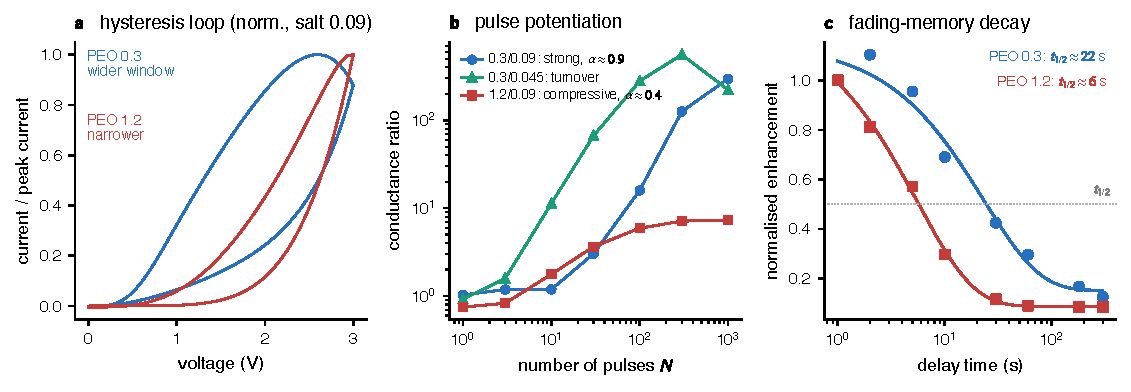
\includegraphics[width=\linewidth]{../figures/chapter4/representative_curves.pdf}
  \caption[Representative raw curves of the three measurements]{Representative raw curves of the three common measurements, on devices chosen near their cell medians (\SY{}/\PEO{}/\LiTf{}/Ag). (a)~Hysteresis loops, each normalised to its own peak current so the comparison is the loop \emph{openness} (the switching window), not absolute conductance: the low-\PEO{} device (\PEO{}~\num{0.3}, blue) opens a wider window than the high-\PEO{} one (\PEO{}~\num{1.2}, red), which carries more current but switches over a narrower range. (b)~Pulse potentiation (conductance ratio vs pulse number, log--log): a strong near-linear accumulation (\(\alpha\approx0.9\)), a low-salt cell that \emph{turns over} and then declines, and a weak, compressive high-\PEO{} response (\(\alpha\approx0.4\)). (c)~Fading-memory decay (enhancement vs delay, normalised to the first read) with stretched-exponential fits and the half-enhancement level dotted: the low-\PEO{} device crosses \(t_{1/2}\) far later (\(\approx\SI{22}{\second}\)) than the high-\PEO{} one (\(\approx\SI{6}{\second}\)).}
  \label{fig:ch4_representative}
\end{figure}

\begin{figure}[t]
  \centering
  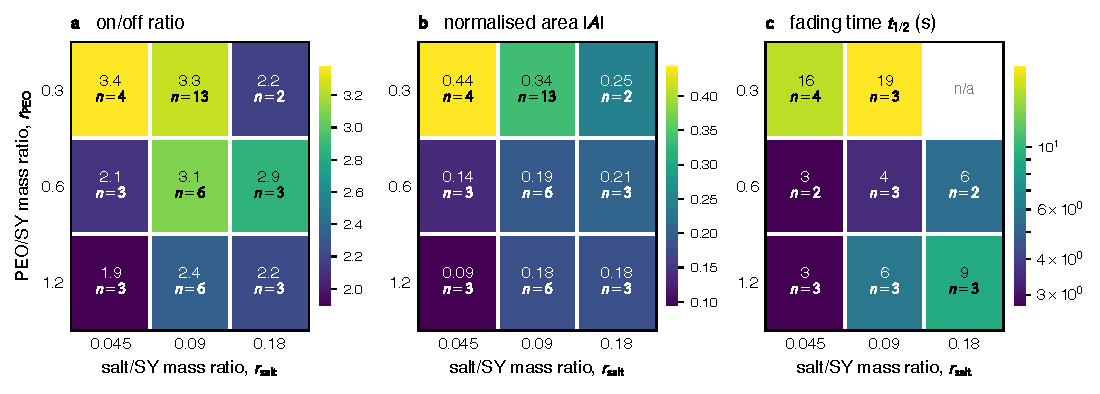
\includegraphics[width=\linewidth]{../figures/chapter4/composition_heatmaps.pdf}
  \caption[Composition control of the memristive dynamics]{Composition control of the steady-state and dynamical response of \SY{}/\PEO{}/\LiTf{} devices. The switching window (a, b) and the fading-memory time (c) both decrease as the \PEO{}-to-\SY{} mass ratio increases at fixed salt ratio.}
  \label{fig:ch4_composition_heatmaps}
\end{figure}

The steady-state switching window contracts as \(r_{\PEO{}}\) rises. At fixed \(r_{\mathrm{salt}}=\num{0.09}\), the median on--off ratio falls from \(\approx 3.3\) at \(r_{\PEO{}}=\num{0.3}\) to \(\approx 2.4\) at \(r_{\PEO{}}=\num{1.2}\), while the normalised loop area falls from \(\approx 0.33\) to \(\approx 0.18\). The activation voltage remains within \SIrange{2.2}{2.4}{\volt} across the grid. Composition thus changes how \emph{much} the conductance moves, but not the voltage at which it begins to move. The widest window occurs in the low-\PEO{} row, with the largest loop area at the low-salt corner (\(r_{\PEO{}}=\num{0.3}\), \(r_{\mathrm{salt}}=\num{0.045}\): area \(\approx 0.44\)). The per-sweep on--off ratio is strongly right-skewed there: the cell median is \(\approx 3.4\), but individual sweeps reach \(\sim 40\). Cell medians are therefore used throughout to prevent these few outlying sweeps from dominating the comparison.

Potentiation also weakens and changes shape with composition (\cref{fig:ch4_potentiation}). The \PEO{} and salt mass ratios affect different features of the response. The per-decade growth of the conductance ratio (the log--log slope $\alpha$) falls with \PEO{} content, most cleanly at the lowest salt ratio. It drops from $\alpha\approx 1.1$ (near-linear accumulation) at \(r_{\PEO{}}=\num{0.3}\) to $\alpha\approx 0.3$ (strongly compressive) at \(r_{\PEO{}}=\num{1.2}\). The usable dynamic range follows the same direction: the peak conductance ratio is largest in the low-\PEO{}, low-salt corner ($\approx 480\times$ at \(r_{\PEO{}}=\num{0.3}\), \(r_{\mathrm{salt}}=\num{0.045}\)) and falls to a few-fold at high \PEO{}. Salt content instead governs how long the response grows before saturation. At the lowest salt ratio (\num{0.045}), every cell \emph{turns over} by $N\sim\numrange{100}{300}$ pulses; at the highest salt ratio (\num{0.18}), the conductance ratio continues to grow through the largest count tested ($N\approx 1000$), with \num{0.09} intermediate. The $\alpha$ trend is noisier at the higher salt ratios, and the sparsely sampled \(r_{\PEO{}}=\num{0.3}\), \(r_{\mathrm{salt}}=\num{0.18}\) cell ($n=2$, curation-recovered) departs from it. Turnover also places a practical ceiling on the usable pulse count. These composition-dependent, predominantly compressive responses provide the nonlinear input encoding used in \Cref{ch:temporal}; the low-salt cells additionally become non-monotone at high pulse counts.

The fading-memory timescale varies with composition over roughly \SIrange{2}{20}{\second}. The longest retention occurs in the low-\PEO{} row (at \(r_{\PEO{}}=\num{0.3}\), \(t_{1/2}\approx\SI{19}{\second}\) at \(r_{\mathrm{salt}}=\num{0.09}\), with an identified \(\tau\approx\SI{25}{\second}\)); increasing \(r_{\PEO{}}\) to \num{0.6} or \num{1.2} shortens the timescale to a few seconds. A single curation-recovered substrate at the still-lower \(r_{\PEO{}}=\num{0.15}\) level (\(t_{1/2}\approx\SI{22}{\second}\)) is consistent with this trend, though it lies outside the replicated grid and is not counted toward it. The independently computed instrument-side single-exponential time constant reproduces the same ordering. Within each cell, the fading-memory time constant varies by \(\sigma(\ln\tau)\approx\num{0.85}\) between nominally identical substrates at fixed composition; film thickness, spin speed, anneal, and device age do not explain this spread (\siCompRef{app:ch4_confounds}; quantified in \cref{app:ch5_scatter}). \Cref{ch:temporal} models the between-cell and within-cell distributions as a heterogeneous bank of fading-memory elements; the range across the whole device library is mapped in \siCompRef{app:ch4_palette}. The same composition axis appears in potentiation strength: the growth exponent \(\alpha\) falls monotonically with \(r_{\PEO{}}\) (cell medians \(\approx0.9\to0.7\to0.35\)), with within-cell variation around each median.

\begin{figure}[t]
  \centering
  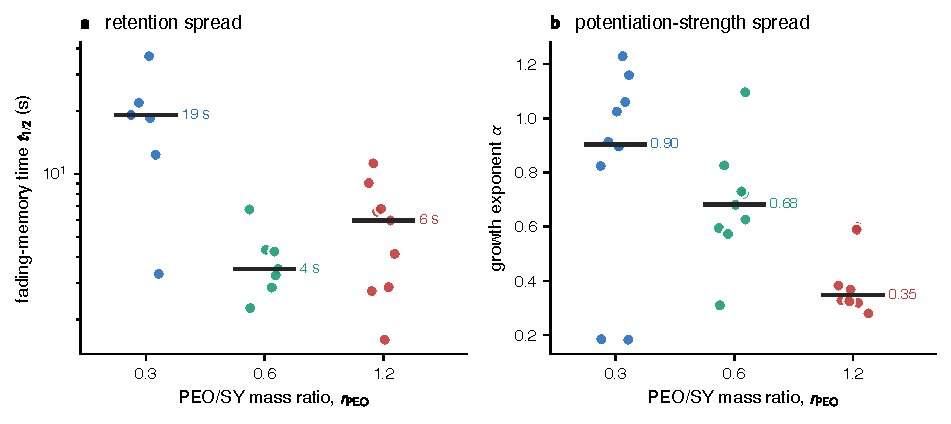
\includegraphics[width=\linewidth]{../figures/chapter4/heterogeneity.pdf}
  \caption[Within-cell substrate-to-substrate heterogeneity]{Per-substrate distributions underlying the cell medians of \cref{fig:ch4_composition_heatmaps} (\SY{}/\PEO{}/\LiTf{}/Ag; black bar is the cell median). (a)~Fading-memory time \(t_{1/2}\) and (b)~potentiation growth exponent \(\alpha\), each against \(r_{\PEO{}}\). The PEO-to-SY mass ratio sets the broad level, while within-cell substrate-to-substrate variation is comparable to the steps between cells. \Cref{ch:temporal} evaluates both sources of variation.}
  \label{fig:ch4_heterogeneity}
\end{figure}

\begin{figure}[t]
  \centering
  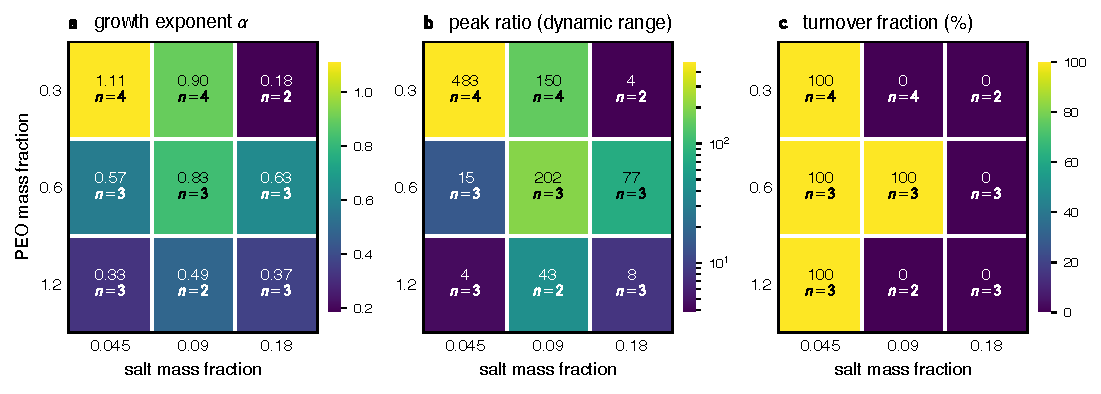
\includegraphics[width=\linewidth]{../figures/chapter4/potentiation_grid.pdf}
  \caption[Composition control of pulse-driven potentiation]{Potentiation (pulse-integration) response across the \SY{}/\PEO{}/\LiTf{} composition grid: (a) the log--log growth exponent $\alpha$, (b) the peak conductance ratio (usable dynamic range, log scale), and (c) the fraction of substrates whose response turns over within the measured range ($N\le 1000$). Increasing \(r_{\PEO{}}\) lowers $\alpha$ and the dynamic range; increasing \(r_{\mathrm{salt}}\) suppresses turnover, sustaining growth to higher pulse counts. Per-cell median, with the substrate count $n$ annotated in each cell.}
  \label{fig:ch4_potentiation}
\end{figure}

Across the replicated grid, increasing the proportion of the ion-transport phase shortens the fading-memory time and is accompanied by smaller switching and potentiation responses, while salt content mainly controls when the response saturates. The \PEO{} gradient is statistically established for the fading-memory time (per-device Spearman \(\rho=-0.52\), permutation \(p=0.009\)); the window and potentiation descriptors move in the same direction but remain marginal (\(p\approx0.06\text{--}0.07\)). A two-way decomposition finds no significant interaction between \PEO{} and salt, and bootstrap confidence intervals on every cell median are given in \siCompRef{app:ch4_gradient}. This replicated composition result is the quantitative core of the chapter; the per-cell values are tabulated in \siCompRef{app:ch4_celltables}. If a more ion-rich matrix relaxes a displaced ionic profile more readily, its equilibrium ionic resistance should also fall. \Cref{sec:ch4_eis} tests that prediction by impedance spectroscopy.

%% ------------------------------------------------------------
\section{Chemical Tuning of the Dynamics}\label{sec:ch4_chemistry}
%% ------------------------------------------------------------

Beyond composition, the identity of the electrolyte components shifts the dynamics further. Each matched cell in this survey (fixed composition, electrode, and protocol) contains at most one or two screened devices. The magnitudes are therefore indicative, and the sample size is given in every case. Structural and optical probes provide a separate view of the chemistry. Blend films and scratched powders at the lead composition (\num{0.3}/\num{0.09}) were examined by ATR-FTIR, X-ray diffraction, and UV-Vis absorption to probe ion association, host backbone order, crystallinity, and the semiconductor's electronic gap without driving a device (\cref{fig:ch4_iratr,fig:ch4_uvvis}). These measurements also use one specimen per chemistry.

\begin{figure}[t]
  \centering
  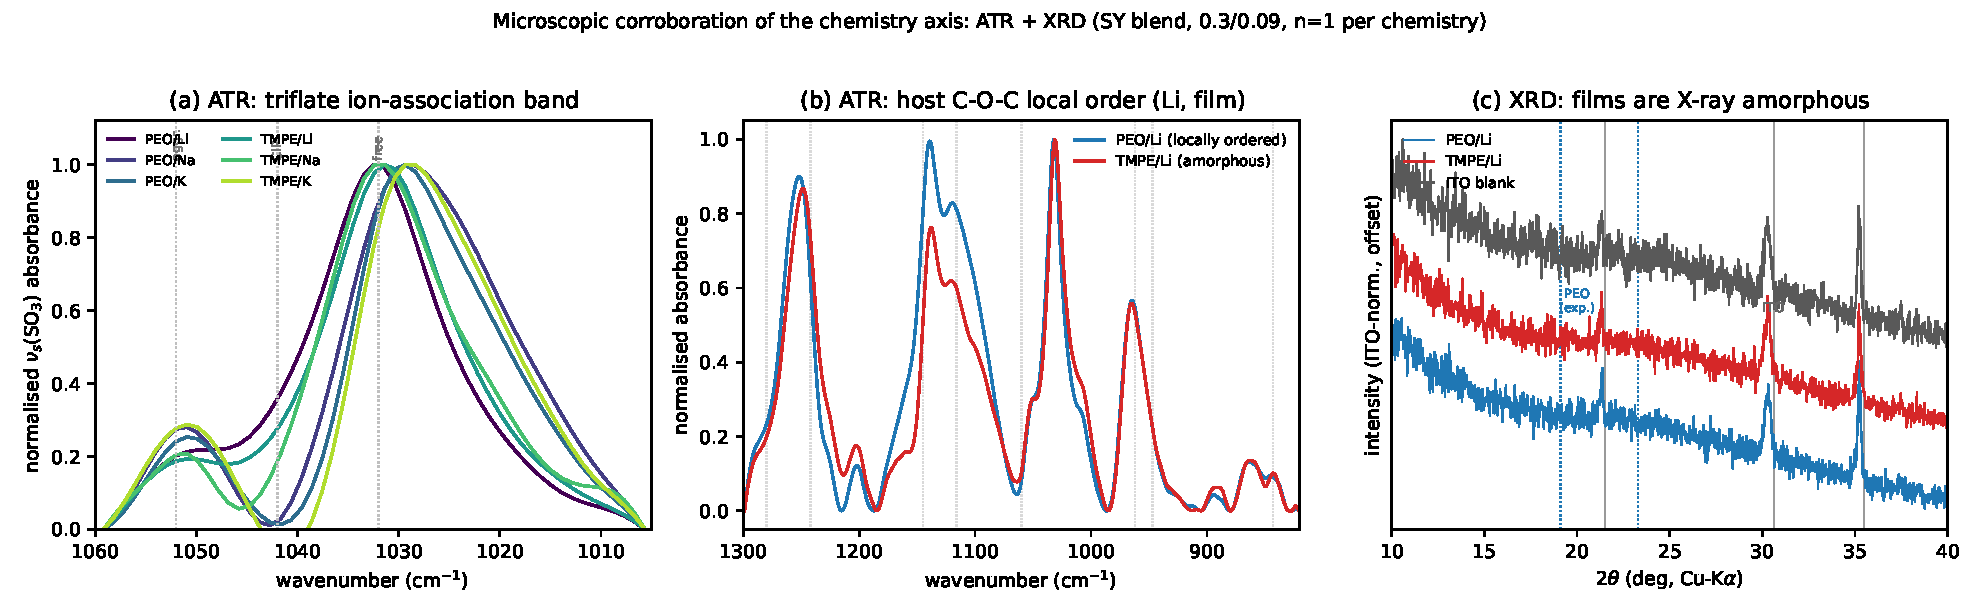
\includegraphics[width=\linewidth]{../figures/chapter4/iratr_chemistry.pdf}
  \caption[Microscopic corroboration of the chemistry axis: ATR and XRD]{Microscopic corroboration of the chemistry axis (electrode-free \SY{}-blend films/powders, \num{0.3}/\num{0.09}, one specimen per chemistry). (a)~ATR-FTIR triflate ion-association band \(\nu_s(\mathrm{SO_3})\), whose position reports the ion-association state (spectroscopically free near \SI{1032}{\per\centi\meter}, contact ion pair near \SI{1042}{\per\centi\meter}, aggregate above; reference positions dotted~\cite{Frech1999PEOLiTf}; \PEO{} hosts in blues, \TMPE{} hosts in reds, darker to lighter for \ce{Li}/\ce{Na}/\ce{K}): it lies at \SIrange{1029}{1032}{\per\centi\meter} in every host\(\times\)cation sample, with no cation-resolved shift. (b)~ATR-FTIR C--O--C envelope: the linear \PEO{} host (blue) shows a resolved multiplet, indicating retained \emph{local} (conformational) ether-backbone order, whereas the hyperbranched \TMPE{} host (red) shows a single broad, amorphous band~\cite{Frech1999PEOLiTf}. (c)~X-ray diffraction of \PEO{}/Li and \TMPE{}/Li with a bare-\ITO{} blank: all patterns show the crystalline \ITO{} substrate reflections (grey lines; \SIlist{21.5;30.6;35.5}{\degree}), with no sharp \PEO{} crystalline doublet (blue dotted; \SIlist{19.1;23.3}{\degree}) or crystalline salt phase. The composite films are therefore X-ray amorphous, and the \PEO{} order in (b) is short-range~\cite{Lightfoot1993,Frech1999PEOLiTf}. ATR spectra are normalised after a local/rubber-band baseline and XRD is normalised to the \ITO{} peak; intensities are not comparable across specimens because sampling and thickness differ, so only band positions and shapes are interpreted.}
  \label{fig:ch4_iratr}
\end{figure}

\begin{figure}[t]
  \centering
  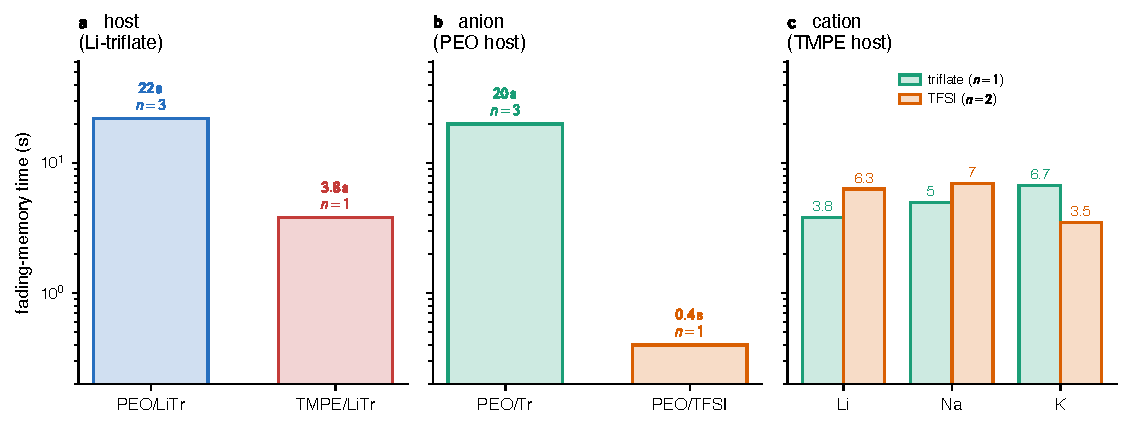
\includegraphics[width=\linewidth]{../figures/chapter4/chemistry_landscape.pdf}
  \caption[Chemistry dependence of the fading-memory time]{Illustrative effect of electrolyte chemistry on the fading-memory time constant (\SY{}, \num{0.3}/\num{0.09}, silver, matched \SI{4}{\volt}/\SI{2}{\volt} protocol). Host (\PEO{} vs \TMPE{}, Li-triflate) and anion (triflate vs \TFSI{}, \PEO{} host) produce the largest shifts. The cation panel shows the same three cations in the \TMPE{} host under each anion: potassium is longest in triflate and shortest in \TFSI{}, so the cation produces no consistent, host- and anion-independent ordering. Sample sizes are small ($n$ as labelled); see text.}
  \label{fig:ch4_chemistry_landscape}
\end{figure}

\paragraph{Host.} Substituting the linear polyether \PEO{} with the hyperbranched polyether \TMPE{}, at fixed lithium-triflate chemistry and composition, shortens the fading-memory time by roughly a factor of six (\PEO{}/\LiTf{}: \(t_{1/2}\approx\SIrange{20}{25}{\second}\), three screened silver devices; \TMPE{}/\LiTf{}: \(\approx\SI{4}{\second}\), one screened silver device with an identified decay). This comparison has three PEO devices but only one TMPE device. The lithium pair from the designed host$\times$cation batch could not be used because the \PEO{}/\LiTf{} device was broken. The analysis therefore compares the \TMPE{} device with the nearest-matched silver \PEO{}/\LiTf{} devices (same operator, fresh semiconductor, glovebox), which differ in fabrication date.

An independent microscopic correlate of the host substitution is visible in the polyether backbone itself, and at two length scales. In ATR-FTIR the linear \PEO{} film shows a resolved C--O--C stretching multiplet, with the weak order-sensitive marker bands near \SIlist{843;962;1242}{\per\centi\meter}, indicating retained \emph{local} (conformational) order of the ether backbone, whereas the hyperbranched \TMPE{} film collapses these into the single broad band of an amorphous polyether (\cref{fig:ch4_iratr}b)~\cite{Frech1999PEOLiTf}. At the longer length scale of crystallites, however, X-ray diffraction on the same sample set finds \emph{neither} host crystalline in the composite: every pattern is dominated by the \ITO{} substrate (confirmed against a bare-substrate blank), with no sharp \PEO{} crystalline reflections and no segregated crystalline salt phase (\cref{fig:ch4_iratr}c), so the films are X-ray amorphous and \PEO{} retains short-range order without forming long-range crystallites~\cite{Lightfoot1993,Frech1999PEOLiTf}. A host that is locally more ordered, even while globally amorphous, set against a fully amorphous \TMPE{}, is consistent with the lower segmental mobility and slower ionic relaxation that the \emph{longer} \PEO{} fading-memory time would require: in polyether electrolytes ion transport is carried by segmental motion of the host above its glass transition, so the relaxation of a displaced ionic profile is rate-limited by that segmental mobility~\cite{Armand1989,RatnerShriver1988,Druger1983}. With one specimen per host this is offered as a structural correlate, not a demonstrated cause. The host ordering is moreover not specific to the silver electrode: on the independent gold-electrode corpus at the same composition, \PEO{} again retains far longer than \TMPE{} and supports a markedly wider switching window and stronger potentiation (\cref{sec:ch4_electrode}), so the host effect survives a change of electrode. That the salt forms no crystalline phase in any chemistry additionally supports reading these blends as homogeneous, salt-dissolved ion-conducting media.

\paragraph{Anion.} Replacing triflate with the more charge-delocalised \TFSI{} anion in the \PEO{} host reduces the fading-memory time from \(\approx\SI{20}{\second}\) to approximately \SI{1}{\second}. This direction is consistent with the electrolyte literature: charge delocalisation in \TFSI{} weakens ion pairing and lowers salt lattice energy, promoting dissociation and plasticisation of the polyether host and increasing ionic mobility~\cite{Vallee1992,BruceVincent1993}. The \TFSI{} decays also tend toward a compressed shape, whereas the triflate decays are stretched, suggesting different relaxation-time distributions. This comparison is weakly controlled: the single \PEO{}/\TFSI{} device belongs to a later fabrication generation and also differs in spin speed and salt filtration. The approximately twenty-fold difference is therefore reported as illustrative.

\paragraph{Cation.} The data do not support the hypothesised \ce{Li+} > \ce{Na+} > \ce{K+} ordering of fading-memory time derived from the hard--soft acid--base argument of \cref{ch:poc}~\cite{Pearson1963}. Two cation series use the same \TMPE{} host, composition, electrode, and protocol, and differ in the salt anion (\cref{fig:ch4_chemistry_landscape}). With triflate, the timescale increases from \ce{Li+} (\(\approx\SI{3.8}{\second}\)) to \ce{Na+} (\(\approx\SI{5.0}{\second}\)) and \ce{K+} (\(\approx\SI{6.7}{\second}\)); each value comes from one screened device with \(R^2\ge0.93\). With \TFSI{}, potassium is shortest (\(\approx\SI{3.5}{\second}\)), while lithium and sodium are longer (\(\approx\SIrange{6}{7}{\second}\), two devices per cation). Thus, cation identity shifts the timescale by roughly a factor of two within a fixed anion, but the ordering changes with the anion and within-cation variation is comparable to between-cation differences. These sample sizes cannot establish a host- and anion-independent ordering. A powered test would require a dedicated series at fixed host, anion, protocol, and electrode with at least three replicates per cell (\cref{sec:ch4_limitations}).

Independent probes provide additional constraints. The triflate symmetric \ce{SO3} stretch \(\nu_s(\mathrm{SO_3})\) lies at \SIrange{1029}{1032}{\per\centi\meter} in all six host\(\times\)cation films and powders, a spread at or below instrumental resolution with no cation ordering (\cref{fig:ch4_iratr}a). UV-Vis absorption of \SY{}/\TMPE{} films places the \SY{} \(\pi\)--\(\pi^{*}\) peak~\cite{Friend1999} at \SI{446}{\nano\meter} for \ce{Li+}, \ce{Na+}, and \ce{K+} (\cref{fig:ch4_uvvis}). These results indicate no resolved cation effect on ion-pairing state or semiconductor optical gap; neither measurement tests the ordering of retention directly. On gold electrodes, the \TMPE{}/triflate steady-state window is also flat across the three cations (on--off ratio \(\approx\numrange{1.3}{1.5}\), no monotone trend; \cref{sec:ch4_electrode}).

\begin{figure}[t]
  \centering
  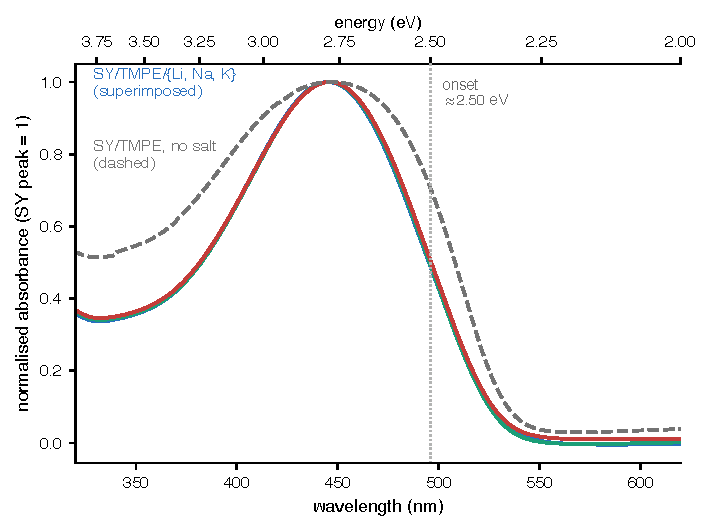
\includegraphics[width=0.56\linewidth]{../figures/chapter4/uvvis_bandedge.pdf}
  \caption[UV-Vis: the \SY{} band edge is invariant to the cation]{UV-Vis absorption of \SY{}/\TMPE{} blend films (lead composition \num{0.3}/\num{0.09}; \ce{Au}-electrode 2025 generation; one specimen per chemistry), normalised to the \SY{} \(\pi\)--\(\pi^{*}\) peak. The peak (\(\approx\SI{446}{\nano\meter}\)) and the absorption onset (\(\approx\SI{2.50}{\electronvolt}\)) are superimposed for \ce{Li+}, \ce{Na+}, and \ce{K+}; the salt-free control (dashed) coincides at the band edge (its differing blue side and lower absolute absorbance are thickness/scattering, not electronic). The cation does not shift the semiconductor's optical gap. Only band \emph{positions} are read because absorbance magnitudes are thickness-confounded.}
  \label{fig:ch4_uvvis}
\end{figure}

In these illustrative comparisons, host and anion substitutions produce larger shifts in fading-memory time than cation substitution.

%% ------------------------------------------------------------
\section{Protocol-Dependent Timescale}\label{sec:ch4_protocol}
%% ------------------------------------------------------------

The drive protocol constrains every comparison above. The read voltage exceeds the ionic activation threshold, and write amplitude controls the displaced ionic profile; both can change the apparent fading-memory time. In one device measured under both protocols, the fitted relaxation time increases from \(\approx\SI{4.6}{\second}\) under a \SI{3}{\volt} write and \SI{1.5}{\volt} read to \(\approx\SI{15.5}{\second}\) under a \SI{6}{\volt} write and \SI{3}{\volt} read (\cref{fig:ch4_protocol}).

\begin{figure}[t]
  \centering
  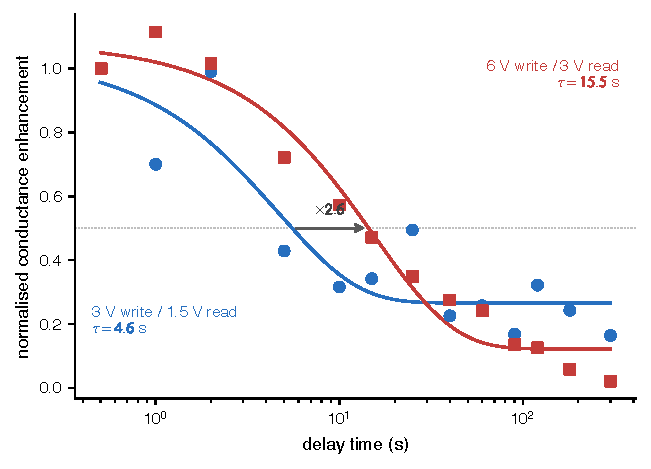
\includegraphics[width=0.62\linewidth]{../figures/chapter4/protocol_overlay.pdf}
  \caption[The drive protocol sets the apparent fading-memory time]{The apparent fading-memory time is set in part by the drive protocol. The same device, measured under a larger write/read amplitude, shows a markedly longer apparent relaxation time: the fitted single-exponential time constant rises from \(\tau\approx\SI{4.6}{\second}\) to \(\approx\SI{15.5}{\second}\), and the half-enhancement crossing (dotted, arrow) shifts by \(\approx\!2.8\times\).}
  \label{fig:ch4_protocol}
\end{figure}

One interpretation is that a larger write amplitude displaces more ionic charge and, at the largest amplitudes, may introduce electrode-level electrochemical processes, producing a longer-lived written state. The supra-threshold read may also perturb the state during interrogation. The composition result of \cref{sec:ch4_composition} remains internally comparable because it uses one fixed protocol. Chemistry comparisons that span device generations are more exposed to protocol differences. Material and drive conditions therefore co-determine the apparent volatile timescale; cross-device or cross-chemistry comparisons must match the write/read protocol, electrode, and composition.

The same lever reappears, independently, on the gold-electrode corpus of \cref{sec:ch4_electrode}. There, matched-amplitude negative pulse trains sweep the pulse count and the inter-pulse interval together, with the relaxation recorded in the same run, and both halves of the protocol dependence are observed directly: potentiation grows steeply as the inter-pulse interval shortens (rank correlation \(\rho\approx-0.94\) to \(-0.99\), \(p<0.001\), in three independent series of \numrange{9}{11} matched runs), and the depth of the written state co-sets the subsequent relaxation time (\(\rho\approx+0.46\) between potentiation ratio and decay half-time, \(p=0.015\), \(n=28\) runs). The drive--retention coupling that this section infers from a two-protocol contrast is therefore seen \emph{within single experiments} on a second electrode (\siCompRef{app:ch4_gold_dynamics}).

%% ------------------------------------------------------------
\section{Microscopic Corroboration: Impedance Spectroscopy}\label{sec:ch4_eis}
%% ------------------------------------------------------------

Every result so far rests on the \emph{driven} response (pulses and decays). Small-signal impedance spectroscopy offers an independent test of the mechanism proposed for the composition trend: if increasing \(r_{\PEO{}}\) shortens the fading-memory time because a more ion-rich matrix lets the displaced ionic profile relax more readily, then the \emph{equilibrium} ionic resistance should fall along the same composition axis. The archive contains such a measurement, acquired on the same substrates: \SI{0}{\volt}-DC spectra (\SI{40}{\milli\volt} AC, \SIrange{1}{1e6}{\hertz}) on \num{26} silver-electrode \SY{}/\PEO{}/\LiTf{} substrates spanning the composition grid.

Each spectrum is summarised in two separate ways. The first is \emph{model-free}: the real part of the impedance at the apex of the main Nyquist semicircle, \(Z_{\mathrm{real}}^{\mathrm{apex}}\), which fixes the resistance scale of the spectrum without committing to any circuit. The second is \emph{model-based}: the bulk ionic resistance \(R_{\mathrm{ion}}\) of an equivalent circuit adapted from the polymer light-emitting electrochemical cell analysis of Munar \textit{et al.}~\cite{Munar2012}, reported only as corroboration of the model-free quantity because the per-spectrum circuit fits are genuinely ill-conditioned. The circuit topology, its two automated fits, and the per-cell values of both observables are detailed in \siCompRef{app:ch4_eis_detail}.

Both observables fall steeply and monotonically with \(r_{\PEO{}}\) (\cref{fig:ch4_eis}a). The model-free \(Z_{\mathrm{real}}^{\mathrm{apex}}\) drops by more than three orders of magnitude across the grid (cell medians from \(\sim\!\SI{e8}{\ohm}\) at \(r_{\PEO{}}=\numrange{0.15}{0.3}\) to \(\sim\!\SI{e5}{\ohm}\) at \(r_{\PEO{}}=\num{1.2}\)), with a rank correlation against \(r_{\PEO{}}\) of \(-0.69\) per substrate (\(n=26\)) and \(-0.83\) on cell medians; the fitted \(R_{\mathrm{ion}}\) gives the same picture (\(-0.84\) on cell medians). This is the direction the mechanism requires: more ion-transport polymer relative to \SY{}, lower ionic resistance.

\begin{figure}[t]
  \centering
  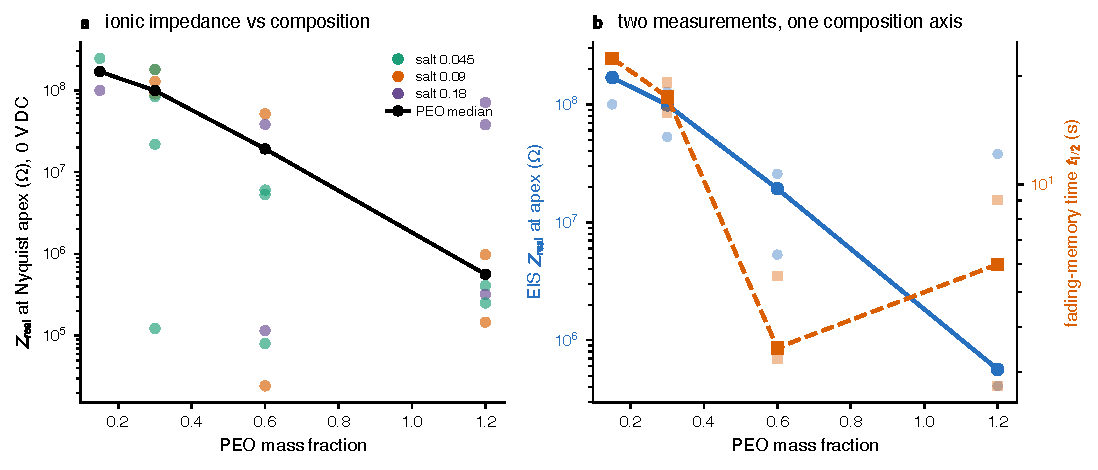
\includegraphics[width=\linewidth]{../figures/chapter4/eis_ionic.pdf}
  \caption[Impedance spectroscopy corroborates the ionic-transport mechanism]{Equilibrium (\SI{0}{\volt}-DC) impedance spectroscopy corroborates the composition control of the dynamics (silver \SY{}/\PEO{}/\LiTf{} grid). (a)~The impedance resistance scale (here the model-free real impedance at the Nyquist apex) falls by more than three orders of magnitude as \(r_{\PEO{}}\) rises (points are substrates, coloured by \(r_{\mathrm{salt}}\); the black line is the \(r_{\PEO{}}\) median). (b)~The equilibrium impedance scale (left axis) and the \emph{independently} measured fading-memory time \(t_{1/2}\) (right axis) decline along the \emph{same} PEO-to-SY composition axis (cell-level points with per-\(r_{\PEO{}}\) median trends): the two are co-driven by composition, not independent variables.}
  \label{fig:ch4_eis}
\end{figure}

The EIS resistance scale and the \emph{independently} measured fading-memory time fall along the \emph{same} composition axis (\cref{fig:ch4_eis}b): both decline together as \(r_{\PEO{}}\) rises, and across cells \(\log Z_{\mathrm{real}}^{\mathrm{apex}}\) covaries with \(\log t_{1/2}\) at \(r\approx+0.74\) (\(+0.61\) per substrate, \(n=23\)). Three qualifications bound this reading:
\begin{itemize}
  \item The PEO-to-SY mass ratio is the \emph{common cause} of both quantities, so this correlation confirms that the same composition axis moves the equilibrium ionic resistance and the driven retention together; it is not evidence of a second, independent factor.
  \item The resistance \emph{scale} carries the composition signal, whereas the EIS relaxation \emph{frequency} does not: the apex frequency corresponds to a sub-second \(RC\) time and does \emph{not} track the seconds-long fading-memory time. This separates the small-signal ionic-transport bottleneck reported by impedance spectroscopy from the slower large-signal relaxation that determines the fading-memory response. The two timescales are nonetheless reconcilable in \emph{magnitude}: the sub-second apex \(RC\) is the geometric-capacitance response, and scaling it by the chemical-to-geometric capacitance ratio measured independently from the low-frequency branch (\(\gtrsim\!33\)) predicts a large-signal relaxation of several seconds, inside the observed \(t_{1/2}\) range (\siCompRef{app:ch4_timescale}).
  \item The effect is not a film-thickness artefact: \(Z_{\mathrm{real}}^{\mathrm{apex}}\) spans \(\sim\!10^{4}\times\) while the film thickness spans only \(2.6\times\), and the \PEO{} dependence survives controlling for thickness (partial correlation \(-0.60\); \cref{sec:ch4_materials}).
\end{itemize}
Impedance spectroscopy thus supplies, for the ionic-resistance half of the mechanistic picture below, the independent microscopic support that the driven measurements alone cannot.

%% ------------------------------------------------------------
\section{Electrode and Polarity Dependence}\label{sec:ch4_electrode}
%% ------------------------------------------------------------

Every result so far uses the silver top electrode. The archive also contains \num{50} gold-electrode devices, treated here as a third illustrative axis. Every gold device uses the single lead composition (\PEO{} or \TMPE{} host, \num{0.3}/\num{0.09}); this corpus therefore contains no information about the composition series of \cref{sec:ch4_composition}, which remains a silver-only result. It instead contrasts electrochemically active silver with inert gold at matched chemistry and provides an independent-electrode check on the chemistry comparisons of \cref{sec:ch4_chemistry}.

At matched chemistry and composition, and under the canonical positive-polarity protocols used everywhere above, the electrode shifts all three behavioural families, and does so coherently (\cref{fig:ch4_electrode}). In the lead \PEO{}/\LiTf{} cell, replacing silver by gold narrows the steady-state switching window (median on--off ratio \(3.3\to2.0\), normalised loop area \(0.33\to0.12\)), weakens and flattens potentiation (peak conductance ratio \(\approx124\times\to29\times\), log--log slope \(\alpha\approx0.9\to0.45\)), and raises the activation voltage (\(\approx\SIrange{2.4}{2.7}{\volt}\)), yet \emph{lengthens} the fading-memory time, from \(t_{1/2}\approx\SI{19}{\second}\) on silver (three devices) to \(\approx\SI{87}{\second}\) on the two clean gold devices (\(R^2\approx0.97\text{--}0.99\), \(\beta\approx0.6\)). The same window-and-potentiation contraction holds in the \TMPE{}/\LiTf{} cell (on--off \(3.8\to1.3\); peak \(54\times\to1.9\times\)), again at positive drive. The per-cell metrics for every chemistry on both electrodes, including the host-free and salt-free negative controls, are tabulated in \siCompRef{app:ch4_electrode_table}.

\begin{figure}[t]
  \centering
  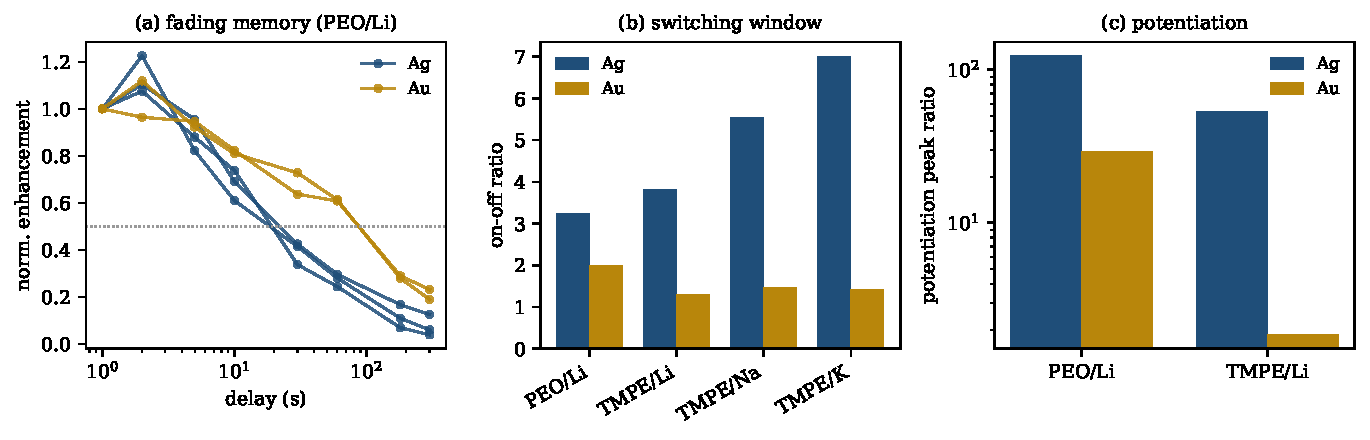
\includegraphics[width=\linewidth]{../figures/chapter4/electrode_contrast.pdf}
  \caption[Electrode dependence: active silver versus inert gold]{Illustrative electrode contrast at the lead composition (\num{0.3}/\num{0.09}), under the canonical positive-polarity protocols (for the negative-polarity behaviour of the gold devices see \cref{fig:ch4_polarity}). (a)~Fading-memory decays of \PEO{}/\LiTf{} devices, normalised to the first read: the gold curves (gold) cross half-enhancement later than the silver ones (blue), i.e.\ gold retains \emph{longer}. (b)~The steady-state switching window (on--off ratio) is narrower on gold for every chemistry, and is flat across the \TMPE{} cation series on gold (no \ce{Li}/\ce{Na}/\ce{K} ordering). (c)~Pulse-potentiation dynamic range (peak ratio, log scale) is far smaller on gold. The inert electrode thus gives a weaker, higher-threshold, but more retentive response. Small $n$ per cell, no human curve curation on the gold side, and a generation offset between the corpora bound the comparison (see text).}
  \label{fig:ch4_electrode}
\end{figure}

This difference is consistent with the contrast between active and inert electrodes. Silver can inject and electrodeposit mobile \ce{Ag+}, the basis of electrochemical-metallisation switching, and may therefore add a large volatile component: a wider window, steeper potentiation, lower threshold, and faster relaxation~\cite{WaserAono2007,Valov2011}. Gold is noble and inert, leaving the polymer-electrolyte ionic mechanism to produce a smaller, higher-threshold, and more persistent response. The higher activation voltage on thinner gold devices supports an interfacial electrode contribution over a film-thickness explanation~\cite{Fang2008}.

\paragraph{Negative-polarity response of the gold devices.} Additional campaigns on the same Au/\TMPE{}/triflate generation measured negative bias. These data were recovered from outside the curated archive and analysed with a dedicated parser; their sources, validation against catalogued sweeps, and per-file tables are documented in \siCompRef{app:ch4_gold_dynamics}. The devices are strongly polarity-asymmetric: within a junction, bipolar sweeps carry \(\approx2.5\)--\(42\times\) more current at \(-3\)~\si{\volt} than at \(+3\)~\si{\volt} (\cref{fig:ch4_polarity}a), with the same direction across the catalogued negative-going sweeps. Under negative drive, the gold devices show a rate-dependent switching window. Across sweep rates of \(\sim\!0.003\)--\(0.4\)~\si{\volt\per\second}, the on--off ratio rises as the sweep slows (rank correlations down to \(-0.99\), \(p<0.001\)), from \(\approx\!1\) at the standard rate to \(\numrange{20}{31}\) in the slowest \(-3\)~\si{\volt} sweeps (\cref{fig:ch4_polarity}b). Constant-bias holds locate an activation threshold between \(-1.5\) and \(-2.5\)~\si{\volt}: current decays below this range and grows by one to three orders of magnitude above it over tens to hundreds of seconds. Negative pulse trains potentiate by one to two orders of magnitude at a matched protocol (\(-5\)~\si{\volt} pulses, \(-2.25\)~\si{\volt} read: cation medians \(\approx40\)--\(230\times\)), while positive pulses depress the written state. The response is therefore bidirectionally programmable under this negative-polarity protocol.

These campaigns add fading-memory measurements for the \TMPE{} host on gold. Sparse delayed reads after the pulse trains, with the device floating between reads, follow strongly stretched exponentials (\(\beta\approx0.33\)--\(0.5\)) with model-free half-decay times of \(\approx\SIrange{0.4}{21}{\second}\) across the three cations (\cref{fig:ch4_polarity}c). These values are on the same seconds scale as \TMPE{} on silver and below the \(\approx\SI{87}{\second}\) measured for \PEO{} on gold, providing a gold-electrode comparison of host retention. Under the matched negative protocol, all three cations have overlapping potentiation ranges and relaxation times, with substrate-to-substrate spread comparable to any cation difference. The concentration of the response in one bias direction after removal of the active \ce{Ag+} pathway is consistent with an interfacial role for the dissimilar ITO and gold contacts and their accumulated ion profiles, but the electrical data do not establish that mechanism.

\begin{figure}[t]
  \centering
  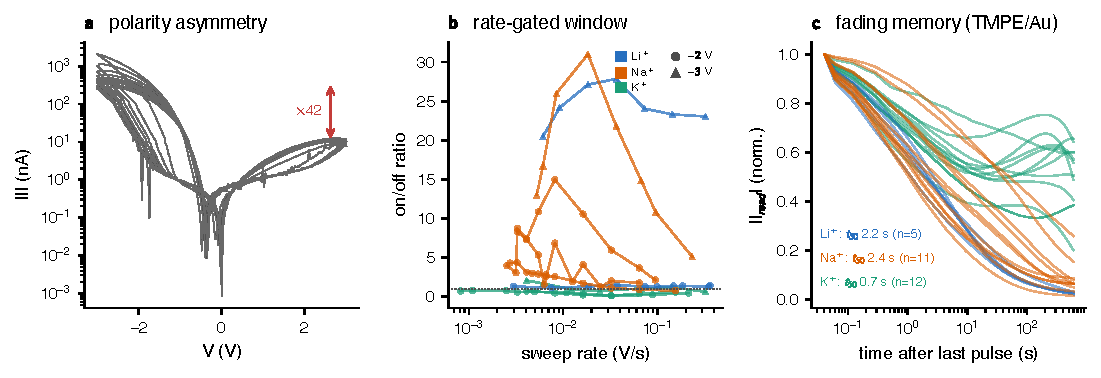
\includegraphics[width=\linewidth]{../figures/chapter4/polarity_dynamics.pdf}
  \caption[Negative-polarity dynamics of the gold/TMPE devices]{Negative-polarity response of the gold/\TMPE{}/triflate devices (illustrative tier; \siCompRef{app:ch4_gold_dynamics}). (a)~Exemplar bipolar sweep (\(\pm3\)~\si{\volt}, ten cycles, Na\(^{+}\) device): the negative branch carries \(\approx42\times\) the current of the positive one. (b)~On--off ratio against sweep rate for all step-count series (colour = cation, marker = amplitude): slow sweeps give ratios of \numrange{20}{31}, while the standard fast protocol gives \(\approx\!1\). (c)~Sparse-read relaxation after \(-5\)~\si{\volt} pulse trains, normalised to the first read, with per-cation median half-decay times. The times are on the seconds scale, as for \TMPE{} on silver, and below those of \PEO{} on gold.}
  \label{fig:ch4_polarity}
\end{figure}

The second electrode reproduces two observations from \cref{sec:ch4_chemistry}: \PEO{} retains longer than \TMPE{}, and the switching window has no transferable cation ordering. The gold corpus also provides negative controls absent from the silver set. Host-free (semiconductor-plus-salt) and salt-free (semiconductor-plus-host) films show neither a switching window (on--off \(\approx1.0\)) nor potentiation (peak \(\approx1\)), indicating that both the ion-transport polymer and dissolved salt are required for the memristive response.

\paragraph{Frequency-domain response: a bias-programmed low-frequency amplifier.} A third corpus measures the same Au/\TMPE{}/triflate chemistry in the frequency domain: \num{549} lock-in sweeps from \SI{1}{\hertz} to \SI{500}{\kilo\hertz} on a fresh batch, with one substrate per cation tracked from day 1 to day 23. The junction is placed in series with a \SI{4}{\nano\farad} capacitor and driven by a small sinusoid superimposed on a programmable DC offset. The apparatus, channel decode, and per-file tables are documented in \siCompRef{app:ch4_lockin}. Above \(\sim\!\SI{10}{\hertz}\), the unbiased junction behaves as a passive linear dielectric: the transfer ratio follows the capacitive divider and is amplitude-independent to within a median \SI{0.2}{\percent} from \num{0.5} to \SI{2.4}{Vpk}. This boundary is consistent with the rate dependence in \cref{fig:ch4_polarity}b. In the same plateau, junction capacitance increases \(\ce{Li}<\ce{Na}<\ce{K}\) by \(\approx\!1.4\times\) across the same-batch trio, compared with an \(\approx\!\SI{1}{\percent}\) pixel spread. Same-recipe profilometry makes a thickness origin less likely, but one substrate per salt limits this result to a candidate dielectric cation effect; profilometry on matched specimens would test it directly. Under DC bias, the fundamental-frequency transfer below \(\sim\!\SI{10}{\hertz}\) increases from \(|H|\approx0.5\) without bias to \(\approx\!18\) at \(\pm\SI{2.5}{\volt}\) (\cref{fig:ch4_lockin}). The bias-modulated ionic conductance transfers energy from the DC offset into the signal band. This gain occurs for all three cations at every age tested, is confined to the sub-\SI{10}{\hertz} band, and is nearly symmetric in bias polarity (\siCompRef{app:ch4_lockin}). A biased junction therefore operates as a voltage-programmable low-pass amplifier over a band that overlaps the physiological signals analysed in \Cref{ch:temporal}.

\begin{figure}[t]
  \centering
  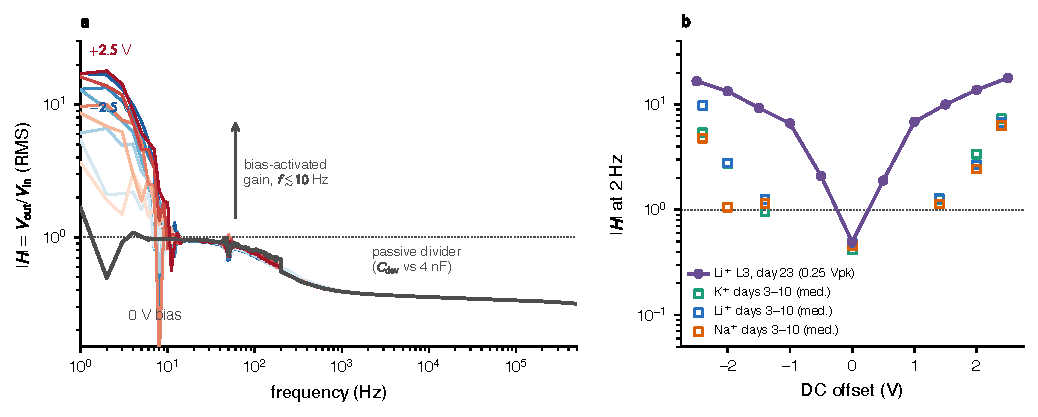
\includegraphics[width=\linewidth]{../figures/chapter4/lockin_response.pdf}
  \caption[Frequency-domain response of the gold/TMPE devices]{Frequency-domain response of the gold/\TMPE{}/triflate devices (illustrative tier; \siCompRef{app:ch4_lockin}). (a)~Transfer ratio \(|H|(f)\) of one \ce{Li+} junction in series with \SI{4}{\nano\farad} (day 23, \SI{0.25}{Vpk}) at eleven DC offsets from \num{0} (grey) to \(\pm\SI{2.5}{\volt}\) (blue negative, red positive). Above \(\sim\!\SI{1}{\kilo\hertz}\), all curves follow the passive capacitive divider; below \(\sim\!\SI{10}{\hertz}\), bias produces a fundamental-frequency gain of up to \(\approx\!18\), increasing with bias magnitude and nearly symmetric in sign. (b)~\(|H|\) at \SI{2}{\hertz} against DC offset for the day-23 series (line) and per-cation medians of earlier sessions (squares; days 3--10, \SIrange{0.4}{1.4}{Vpk}). Gain increases with bias and occurs for all three cations.}
  \label{fig:ch4_lockin}
\end{figure}

All three gold corpora share the same illustrative-tier bounds, which the SI states for each corpus (\siCompRef{app:ch4_gold_dynamics,app:ch4_lockin}). Each uses the single lead composition on one or two substrates per cation; the curves are uncurated; and the supra-threshold negative read makes decay times protocol-specific, allowing only order-of-magnitude comparison with silver. The 2024--2025 gold generation is also partly confounded with electrode because the silver chemistry was fabricated earlier and the co-fabricated silver batch was not measured under the decay protocol. Electrode and polarity are therefore treated as illustrative effects and cross-electrode checks on the chemistry axis. A matched-generation batch split between silver and gold is required for a quantitative electrode comparison.

%% ------------------------------------------------------------
\section{Discussion}\label{sec:ch4_discussion}
%% ------------------------------------------------------------

Composition is the only replicated axis for control of the volatile dynamics. Increasing the ion-transport-polymer-to-semiconductor mass ratio shortens the fading-memory time and is accompanied by smaller switching and potentiation responses. Host and anion substitutions shift the timescale over a wider range, but those comparisons are illustrative. Cation identity also shifts the dynamics, although the direction changes with host, anion, and protocol at the available sample sizes; the predicted \ce{Li+}>\ce{Na+}>\ce{K+} order is therefore not transferable across the dataset.

The electrode acts jointly with drive polarity. Relative to active silver, inert gold weakens switching and potentiation and lengthens retention under the canonical positive drive. Under negative drive, the same gold devices show a full, rate-gated, bidirectionally programmable response (\cref{sec:ch4_electrode}). The frequency measurements locate the corresponding spectral boundary: above \(\sim\!\SI{10}{\hertz}\) the gold junctions behave as passive linear capacitors at every tested amplitude, whereas a DC bias produces programmable low-frequency gain below that boundary.

The hard--soft acid--base model of \cref{ch:poc} remains a qualitative interpretation. It anticipates the cation ordering in the \TFSI{} family, where the most weakly coordinating cation relaxes fastest, but the triflate family runs in the opposite direction. The present data therefore do not support a quantitative cation law.

\paragraph{Mechanistic interpretation.} The mechanism remains a hypothesis. Increasing \(r_{\PEO{}}\) does not produce the decrease in absolute on-state conductance expected from simple dilution of the \SY{} percolation pathway; instead, on-state conductance rises by more than three orders of magnitude across the grid (\siCompRef{app:ch4_percolation}). A rising conductance floor is consistent with the contracting window: the ion-rich phase may add a parallel, weakly switchable path, with off-state conductance rising faster than on-state conductance. Faster relaxation of the displaced ionic profile could account for the accompanying decrease in fading-memory time. Salt content may set the number of mobile, chargeable states available before saturation, consistent with the later turnover at higher \(r_{\mathrm{salt}}\).

Host and anion effects may arise from cation--ether coordination, ion pairing, and segmental mobility~\cite{RatnerShriver1988,BruceVincent1993}, which set the distribution of local activation barriers behind stretched-exponential relaxation~\cite{Sturman2003}. Equilibrium impedance supports the ionic-resistance part of this interpretation: it falls along the composition axis and tracks the fading-memory time (\cref{sec:ch4_eis}). ATR associates the host effect with local ether-backbone order, retained in \PEO{} and absent in amorphous \TMPE{}, while XRD shows that every composite remains X-ray amorphous and that the salt is dissolved rather than segregated. Across the cation series, ATR shows no corresponding ion-association fingerprint and UV-Vis shows no shift of the \SY{} optical gap (\cref{sec:ch4_chemistry}). These measurements are consistent with electrolyte-controlled ion transport rather than a change in the \SY{} electronic backbone.

The anion and barrier-distribution links have not been established microscopically. They require temperature-dependent relaxation measurements and chemistry-resolved impedance (\cref{sec:ch4_limitations}), so the hard--soft acid--base interpretation remains qualitative.

The measured spread of fading-memory times can populate a physical reservoir with distinct temporal responses~\cite{BoydChua1985,Maass2002LSM,Tanaka2019}. Across compositions and nominally identical substrates, the timescale spans roughly an order of magnitude. A two-\(\sigma\) criterion on the cell-median span of \(\Delta\ln t_{1/2}\approx2.1\), relative to within-cell scatter, resolves approximately two to five composition bands (\siCompRef{app:ch4_resource}). Each junction reproduces its switching window to \(\approx\SI{15}{\percent}\) sweep-to-sweep (\siCompRef{app:ch4_reproducibility}), substantially less than the diversity across the bank. \Cref{fig:ch4_design_space} places every screened silver substrate in a fading-memory (\(t_{1/2}\)) versus dynamic-range (peak ratio) plane. The PEO-to-SY mass ratio sets the broad region occupied by each substrate, so one composition selects a paired memory/nonlinearity operating point; the remaining within-composition scatter supplies additional substrate-to-substrate diversity. \Cref{ch:temporal} evaluates both sources of variation.

\begin{figure}[t]
  \centering
  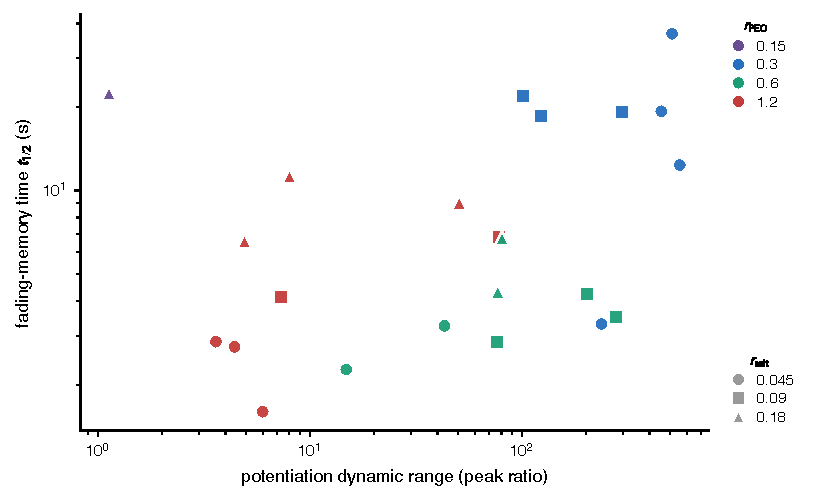
\includegraphics[width=0.6\linewidth]{../figures/chapter4/design_space.pdf}
  \caption[Per-substrate design space]{Per-substrate design space of the \SY{}/\PEO{}/\LiTf{}/Ag composition grid: fading-memory time $t_{1/2}$ against potentiation dynamic range (peak ratio), coloured by \(r_{\PEO{}}\) and marked by \(r_{\mathrm{salt}}\) (one point per fabricated substrate, median over its junctions). The \PEO{} ratio selects the broad region a substrate occupies: low \PEO{} (blue) in the long-memory, high-dynamic-range corner, high \PEO{} (red) in the opposite one, so memory and nonlinearity are \emph{paired}, not independently tunable. The substantial within-composition scatter is the genuine substrate-to-substrate heterogeneity that \Cref{ch:temporal} exploits.}
  \label{fig:ch4_design_space}
\end{figure}

%% ------------------------------------------------------------
\section{Limitations and Future Work}\label{sec:ch4_limitations}
%% ------------------------------------------------------------

Statistical power is limited outside the composition axis. Only the \SY{}/\PEO{}/\LiTf{} composition grid is replicated; the host, anion, and cation comparisons rest on one or two screened devices per matched cell.
\begin{enumerate}
  \item The cation hypothesis is not tested here at adequate power. The cation does shift the dynamics, but not as predicted: the triflate retention series runs \ce{K}>\ce{Na}>\ce{Li}, the reverse of the hypothesised \ce{Li+}>\ce{Na+}>\ce{K+}, and re-orders again with the anion, so the hypothesised ordering is not what the data show and no transferable cation law can be fixed at one or two devices per cell.
  \item The supra-threshold read and the amplitude dependence of the apparent timescale (\cref{sec:ch4_protocol}) mean that absolute retention values are protocol-specific.
  \item The electrode is reported as an illustrative axis (\cref{sec:ch4_electrode}), but it remains partly confounded with fabrication generation, and device ageing is an uncontrolled variable that was not modelled.
  \item Pulse integration and state relaxation were characterised \emph{separately and at different write amplitudes}: the potentiation curves used a \SI{3}{\volt} write and the fading-memory decays a \SI{4}{\volt} write (\cref{tab:ch4_protocols}), at an effectively common inter-pulse interval. On the lead silver composition, the archive contains no experiment that varies input timing to probe their interaction directly. A matched-amplitude experiment exists on the gold/\TMPE{} corpus (\cref{sec:ch4_electrode}), but it uses a different host, electrode, polarity, and read, so it establishes the direction of coupling rather than the lead-cell parameters.
  \item The fading-memory protocol measured a single junction per device, so repeat-decay reproducibility of \(t_{1/2}\) is not characterised at the population level (only one device carries two junctions; \siCompRef{app:ch4_reproducibility}). Within-device reproducibility is established only for the steady-state switching window, from its repeated sweeps.
\end{enumerate}
Because drive amplitude affects the apparent timescale (\cref{sec:ch4_protocol}), combining the \SI{3}{\volt} potentiation shape with the \SI{4}{\volt} decay in \Cref{ch:temporal} requires an explicit modelling assumption that the regimes are compatible. A matched-amplitude experiment that varies both pulse count and inter-pulse interval would test this assumption. Its gold/\TMPE{} negative-polarity counterpart shows coupling between the two measurements (\cref{sec:ch4_protocol}); the lead-composition silver experiment remains future work.

A dedicated cation series in one host and anion, at a fixed protocol and electrode, with a sub-threshold read voltage (as in \cref{ch:poc}) and at least three replicates per cell, would turn the illustrative chemistry survey into a powered comparison. The impedance study of \cref{sec:ch4_eis} could also be extended beyond the replicated \PEO{}/\LiTf{} axis at \SI{0}{\volt} DC. The archive contains unmodelled bias-resolved spectra up to \SI{3}{\volt} DC and chemistry-varied devices; analysing them would test the proposed host, anion, and barrier-distribution effects. A matched-generation batch split between silver and gold top electrodes would isolate the electrode effect from fabrication generation.

Temperature-dependent relaxation measurements are needed to test the proposed role of segmental mobility and distributed activation barriers. A \(\tau(T)\) series yielding an Arrhenius or Vogel--Fulcher--Tammann activation energy would connect the host and anion differences to a segmental-relaxation barrier and test the temperature dependence of the stretch exponent \(\beta\). Encapsulation and systematic ageing measurements would address the remaining stability questions.

%% ------------------------------------------------------------
\section{Inputs to Temporal Computing}\label{sec:ch4_bridge}
%% ------------------------------------------------------------

In the replicated \SY{}/\PEO{}/\LiTf{} grid, composition tunes the fading-memory time over roughly \SIrange{2}{20}{\second}, with the switching window and potentiation strength moving in the same direction. Host and anion contrasts extend the measured range, although each rests on at most one or two devices per matched cell. Cation identity also shifts the dynamics, but the available data do not establish the predicted \ce{Li+}>\ce{Na+}>\ce{K+} order as a transferable law. Drive protocol co-sets the apparent timescale and must remain fixed in quantitative comparisons.

\Cref{ch:temporal} uses the fading-memory times and substrate-to-substrate variability measured in this chapter. It also uses the pulse-update curves, including their saturation and turnover. Because \(r_{\PEO{}}\) changes both the fading-memory time and the input nonlinearity \(\alpha\) (\cref{fig:ch4_design_space}), each composition defines a paired operating point rather than two independent settings. The salt-to-SY mass ratio provides a partly separate control of dynamic range and turnover. The simulations therefore compare banks drawn from one composition with banks spanning several compositions.


%% ---- Standalone close (skipped when \include'd from thesis.tex) ----
%% A unified bibliography is printed from thesis.tex in the thesis build,
%% so the per-chapter \printbibliography runs only in standalone mode.
\ifdefined\thesismode
  \let\thesisstandaloneclose\relax
\else
  \printbibliography[heading=bibintoc, title={References}]
  \def\thesisstandaloneclose{\end{document}}
\fi
\thesisstandaloneclose
